% Satelliittien ylilentoennuste: selitys.
% Käännös: tectonic docs/pass_prediction_explained_fi.tex   (tuottaa docs/pass_prediction_explained_fi.pdf)
\documentclass[a4paper,11pt]{article}

\usepackage{fontspec}
\usepackage[finnish]{babel}
\usepackage{amsmath,amssymb}
\usepackage{icomma}            % desimaalipilkku matematiikassa: 0,9233
\usepackage[margin=2.5cm]{geometry}
\usepackage{booktabs,tabularx,array}
\usepackage{graphicx}
\usepackage{enumitem}
\usepackage{xcolor}
\usepackage{tikz}
\usetikzlibrary{angles,quotes,babel}  % babel: Finnish makes " active
\usepackage[hidelinks]{hyperref}

\setlist{itemsep=2pt,topsep=4pt}
\setlength{\emergencystretch}{2em}  % avoid overfull lines with long Finnish words
\newcommand{\unverified}[1][]{\textcolor{gray}{\texttt{[unverified#1]}}}
\newcommand{\koodi}[1]{\texttt{#1}}
\newcolumntype{L}{>{\raggedright\arraybackslash}X}

\title{Satelliittien ylilentoennuste: selitys}
\author{Projektin \koodi{passplan} oppimateriaali}
\date{31.10.2026, päivitetty 12.11.2026}

\begin{document}
\maketitle

Tämä dokumentti selittää, mitä ylilentoennusteen takana on: mistä ratatiedot tulevat, miten satelliitin paikka lasketaan, miten se muunnetaan maa-aseman taivaalle ja mitä tuloksista voi päätellä. Taustaksi riittävät fysiikan perusteet (vektorit, trigonometria, Newtonin mekaniikka). Dokumentin on kirjoittanut tekoälyagentti (Claude Code) osana projektia.

\paragraph{Lähteiden merkintä.} Kun väite tulee lähteestä, lähde on suluissa. Tässä projektissa on luettu nämä:
\begin{itemize}
  \item \emph{Vallado, Crawford, Hujsak \& Kelso (2006)}, ”Revisiting Spacetrack Report \#3”, AIAA 2006-6753. PDF luettu 31.10.2026.
  \item \emph{Skyfield-dokumentaatio}, sivu ”Earth Satellites”, luettu 31.10.2026. Lisäksi on luettu Skyfieldin 1.54-version lähdekoodia.
  \item \emph{CelesTrak}, sivut ”A New Way to Obtain GP Data” ja ”Usage Policy”, luettu 31.10.2026, ja etusivu, luettu 5.11.2026.
  \item \emph{sgp4-kirjaston lähdekoodi}, versio 2.26 (tiedostot \koodi{omm.py} ja \koodi{alpha5.py}), luettu 5.11.2026.
  \item \emph{Wikipedia}, artikkelit ”Two-line element set” ja ”Simplified perturbations models”, luettu 31.10.2026. Ne ovat toissijaisia lähteitä, ja ne on merkitty sellaisiksi.
\end{itemize}
\unverified{} tarkoittaa, että tieto on yleisesti tunnettua, mutta sitä ei tarkistettu lähteestä tämän työn aikana.

\tableofcontents

%----------------------------------------------------------------------
\section{Käyttö lyhyesti}\label{sec:kaytto}

Paketissa \koodi{passplan} on kolme komentoa. Ne ajetaan Pythonin \koodi{-m}-valitsimella,
joka ajaa paketin tai sen moduulin ohjelmana. Esimerkiksi \koodi{python -m passplan} ajaa
paketin pääohjelman eli tiedoston \koodi{passplan/\_\_main\_\_.py}, ja
\koodi{python -m passplan.schedule} ajaa tiedoston \koodi{passplan/schedule.py}.
\begin{itemize}
  \item \koodi{python -m passplan}: yhden satelliitin ylilennot yhdeltä asemalta (tämä luku).
  \item \koodi{python -m passplan.schedule}: usean satelliitin yhteysaikataulu yhdelle
    antennille (luku~\ref{sec:aikataulu}).
  \item \koodi{python -m passplan.heavens\_above}: avaa Heavens-Aboven ylilentolistan samalle
    paikalle vertailua varten (luku~\ref{sec:vertailu}).
\end{itemize}
Jokainen komento listaa omat valitsimensa, kun sille antaa valitsimen \koodi{--help}.

Ohjelma ajetaan projektikansiosta (GitHubista kloonattuna \koodi{satellite-pass-planner})
ympäristössä \koodi{passplan}:
\begin{verbatim}
conda activate passplan
cd satellite-pass-planner
python -m passplan --norad 25544
python -m passplan --name "cosmos 1833" --station koti \
    --min-elevation 0 --visibility
python -m passplan --norad 17589 --station koti --days 1 --plot pass_koti.png
\end{verbatim}

\noindent Valitsimet:
\begin{center}
\begin{tabularx}{\textwidth}{@{}lL@{}}
\toprule
Valitsin & Merkitys \\
\midrule
\koodi{--norad N} & NORAD-numero (5 tai 6 numeroa); ratatiedot haetaan CelesTrakista
  OMM-muodossa ja pidetään välimuistissa 2\,h. \\
\koodi{--name TEKSTI} & Haku nimen osalla. Yksi osuma lasketaan suoraan, useampi listataan
  NORAD-numeroineen. \\
\koodi{--tle-file TIEDOSTO} & TLE- tai OMM/JSON-tiedosto (toimii ilman verkkoa). \\
\koodi{--cache-dir KANSIO} & Ratatietojen ja efemeridin välimuisti; oletus \koodi{.tle\_cache}. \\
\koodi{--station NIMI} & \koodi{helsinki} (Tähtitorninvuori), \koodi{turku} (Kauppatori) tai oma
  yksityinen asema, esim.\ \koodi{koti}. Oletus on Helsinki, ellei omassa asematiedostossa
  ole muuta oletusta. \\
\koodi{--lat}, \koodi{--lon}, \koodi{--altitude-m} & Mikä tahansa muu paikka (asteina, metreinä;
  korkeuden oletus 0\,m). Ohittaa valitsimen \koodi{--station}. \\
\koodi{--start}, \koodi{--days} & Hakuikkuna; oletus nyt + 2 vrk. \koodi{--start} ilman
  aikavyöhykettä on UTC. \\
\koodi{--min-elevation} & Horisonttimaski asteina; oletus 10. \\
\koodi{--plot}, \koodi{--plot-pass N} & Taivaskuva PNG-tiedostoon. Pelkkä tiedostonimi
  tallentuu kansioon \koodi{plots/}. \\
\koodi{--visibility} & Näkyykö ylilento silmällä (luku~\ref{sec:nakyvyys}). Lataa
  ensimmäisellä kerralla 17\,MB:n DE421-efemeridin välimuistiin. \\
\koodi{-h}, \koodi{--help} & Valitsimet ja niiden oletusarvot. \\
\bottomrule
\end{tabularx}
\end{center}

\subsection{Oma kotiasema}
Paikat, joita ei haluta versionhallintaan, ovat tiedostossa
\koodi{\textasciitilde/.config/passplan/stations.json} projektikansion ulkopuolella.
Ympäristömuuttuja \koodi{PASSPLAN\_STATIONS} voi osoittaa toiseen tiedostoon.
Tiedostoa voi muokata esimerkiksi komennolla
\begin{verbatim}
nano ~/.config/passplan/stations.json
\end{verbatim}
Muoto:
\begin{verbatim}
{
  "default": "koti",
  "stations": {
    "koti": {"name": "Koti", "latitude_degrees": 60.0,
             "longitude_degrees": 22.0, "altitude_m": 5}
  }
}
\end{verbatim}
Kenttä \koodi{"default"} on vapaaehtoinen; ilman sitä oletusasema on Helsinki.
Tulosteessa näkyy vain aseman nimi, ei koordinaatteja, joten tulosteen voi jakaa.

\subsection{Yhteysaikataulu: \koodi{passplan.schedule}}\label{sec:aikataulu}
Maa-asemalla on usein monta satelliittia, mutta antenni voi seurata vain yhtä kerrallaan.
\koodi{python -m passplan.schedule} laskee annettujen satelliittien ylilennot yhdeltä
asemalta ja valitsee niistä ne, jotka yksi antenni ehtii palvella. Satelliitit annetaan
tärkeysjärjestyksessä: ensimmäinen \koodi{--satellite} on tärkein (P1), toinen P2 ja niin
edelleen. Esimerkki (ISS tärkein, sitten NOAA 20 ja Sentinel-6A):
\begin{verbatim}
python -m passplan.schedule --satellite 25544 --satellite 43013 \
    --satellite 46984 --days 1
\end{verbatim}

\noindent Valitsimet:
\begin{center}
\begin{tabularx}{\textwidth}{@{}lL@{}}
\toprule
Valitsin & Merkitys \\
\midrule
\koodi{--satellite X} & NORAD-numero tai TLE- tai OMM/JSON-tiedosto. Toistetaan jokaiselle
  satelliitille; järjestys on prioriteetti. \\
\koodi{--station NIMI} & Kuten yllä. \\
\koodi{--start}, \koodi{--days} & Hakuikkuna; oletus nyt + 1 vrk. \\
\koodi{--min-elevation} & Horisonttimaski asteina; oletus 10. \\
\koodi{--slew-minutes} & Antennin kääntöaika yhteyksien välissä minuutteina; oletus 2. \\
\koodi{--cache-dir} & Kuten yllä. \\
\bottomrule
\end{tabularx}
\end{center}

\paragraph{Valintasääntö.} Sääntö on ahne (\emph{greedy}): ehdokkaat käydään läpi
järjestyksessä, ja kukin hyväksytään tai hylätään lopullisesti.
\begin{enumerate}
  \item Tärkeämpi satelliitti ensin.
  \item Saman prioriteetin sisällä korkeimmalle nouseva ylilento ensin: se kestää
    pidempään ja satelliitti on lähempänä, joten dataa siirtyy enemmän.
  \item Tasatilanteessa aikaisempi, jotta tulos on joka ajolla sama.
\end{enumerate}
Ehdokas hyväksytään, jos sen AOS on vähintään kääntöajan verran jokaisen aiemman hyväksytyn
yhteyden LOS:n jälkeen ja sen LOS vähintään kääntöajan verran ennen jokaista myöhempää.
Muuten se hylätään, ja syy nimeää yhteyden, joka esti sen.

\paragraph{Tuloste.} Viiden satelliitin esimerkki testidatasta (README:ssä sama komento):
{\small
\begin{verbatim}
Scheduled contacts (28, total 3 h 21 min 32 s):
+ ISS (ZARYA) (P1)       11-01 00:42:50-00:47:54 UTC [02:42 EET]  max el 19.6°
+ NOAA 20 (JPSS-1) (P5)  11-01 01:04:57-01:15:44 UTC [03:04 EET]  max el 74.2°
...
Rejected contacts (4):
- SENTINEL-2A (P4)       11-01 08:49:01-08:58:51 UTC [10:49 EET]  max el 40.6°
    reason: only 0.4 min apart from higher-ranked contact SENTINEL-2B (P2) ...
\end{verbatim}
}
\noindent Rivit, joiden alussa on \koodi{+}, ovat aikatauluun otetut yhteydet; \koodi{-}-rivit
on hylätty. Aika on muodossa kuukausi-päivä ja AOS--LOS (UTC), hakasulkeissa AOS Suomen
aikaa ja lopussa huippukorkeus. Sentinel-2A ja -2B kiertävät samaa rataa puolen kierroksen
päässä toisistaan, joten niiden ylilennot tulevat minuuttien välein, ja yhdellä antennilla
vähemmän tärkeä kaksonen jää ilman.

\paragraph{Mitä yksinkertaistus jättää pois.} Ahne sääntö ei ole paras mahdollinen: yksi
korkea ylilento voi estää kaksi lyhyempää, jotka yhdessä toisivat enemmän dataa. Oikeat
maa-asemaverkot ratkaisevat aikataulun optimointina, ja rajoitteina on muun muassa useita
antenneja ja asemia, osittaisia yhteyksiä, datamäärät ja satelliitin muisti, linkkibudjetti
(datanopeus riippuu korkeudesta ja etäisyydestä) sekä todellinen, kääntökulmasta riippuva
kääntöaika. Ikkunan lopussa katkeava ylilento otetaan aikatauluun sellaisenaan, ilman
merkintää.

\subsection{Vertailu muihin ohjelmiin}\label{sec:vertailu}
Heavens-Above ja Sky Safari laskevat ylilennot samoista julkisista ratatiedoista ja
todennäköisesti samalla SGP4-mallilla. Vertailu tarkistaa siis laskentaketjun (paikka,
koordinaatistot, tapahtumahaku), ei sitä, kuinka tarkasti ratatieto kuvaa todellista rataa.
Vertailussa neljä asiaa ratkaisee.

\paragraph{Horisonttiraja (\koodi{--min-elevation}).}
\begin{itemize}
  \item \textbf{Oletus $10^\circ$.} AOS ja LOS ovat hetkiä, jolloin satelliitti ylittää
    $10^\circ$:n korkeuden. Esimerkki 2.11.2026: Cosmos 1833 laski Turun Kauppatorilta
    katsottuna $10^\circ$:n alle klo 19.46.23 mutta horisonttiin vasta 19.48.48 (Suomen aikaa),
    ero 2\,min 25\,s.
  \item \textbf{Heavens-Above: \koodi{--min-elevation 0}.} Heavens-Above antaa nousun ja
    laskun geometrisessa horisontissa. Sen ylilentolista näyttää oletuksena vain ylilennot,
    jotka nousevat vähintään $10^\circ$:een: Sentinel-6A:n ylilento 12.11.2026 klo 06.52 UTC
    puuttui Kauppatorin listasta, ja tämän ohjelman mukaan sen huippu oli $9{,}69^\circ$.
    Ylilennon omalta sivulta saa sekä $0^\circ$:n että $10^\circ$:n ajat.
  \item \textbf{Sky Safari: \koodi{--min-elevation -0.57}.} Sky Safari antaa nousun ja laskun
    hetkellä, jolloin geometrinen korkeus on $-34'$. Se on tähtitieteen tavallinen nousun
    määritelmä, joka ottaa huomioon ilmakehän taittumisen horisontissa. Matalalla
    Sentinel-6A:n ylilennolla ero $0^\circ$:n aikoihin oli 17\,s sekä nousussa että laskussa;
    $-0{,}57^\circ$:n rajalla ajat täsmäsivät sekunnilleen. Huippukorkeudet ja suunnat voi
    verrata suoraan, sillä ne vastasivat ohjelman geometrisia arvoja (päätelty vertailuista,
    ei tarkistettu Sky Safarin dokumentaatiosta).
\end{itemize}

\paragraph{Ikkunan alku.} Ilman \koodi{--start}-valitsinta ikkuna alkaa ajohetkestä. Jos
satelliitti on silloin jo taivaalla, ylilento on katkaistu: tuloste merkitsee AOS:n tekstillä
”window start” ja MAX:n tekstillä ”highest point inside window”. Silloin MAX on ikkunan
korkein kohta, ei koko ylilennon huippu. Ikkunan voi aloittaa ennen ylilentoa, esimerkiksi
\koodi{--start 2026-11-12T08:15:00+02:00} (Suomen aika) tai \koodi{--start 2026-11-12T06:15:00}
(UTC; aika ilman aikavyöhykettä on UTC).

\paragraph{Sekunnit.} Ohjelma katkaisee ajat kokonaisiksi sekunneiksi (20.08.48,82
tulostuu 20.08.48), ja Heavens-Above näyttää tekevän samoin. Tapahtumahaku on muutaman
sekunnin kymmenyksen tarkka: ISS:n laskulle Helsingissä 12.11.2026 haku antoi 40~eri
ikkunan alulla ajan väliltä 20.08.48,821--48,867, ja tiheä näytteistys antoi 48,822. Yhden
sekunnin ero tulosteissa on siksi mahdollinen, kun todellinen aika on lähellä täyttä sekuntia.

\paragraph{Ratatiedon ikä.} Tulosteen \koodi{Epoch}-rivi kertoo, minkä hetken rataa
ratatieto kuvaa, ja \koodi{Retrieved}-rivi, milloin ohjelma haki sen. Vertailussa kummankin
ohjelman ratatietojen pitää olla tuoreita; Sky Safarin ratatiedot päivittyvät vain sen omasta
päivityspainikkeesta.

\subsubsection*{Heavens-Above-linkit}
Heavens-Aboven valikoista löytyvät vain kirkkaimmat satelliitit, mutta minkä tahansa
satelliitin ylilentolistan saa osoitteella. Valmiit linkit tämän ohjelman asemille, samoilla
koordinaateilla:
\begin{itemize}
  \item Turku, Kauppatori:\\
    \url{https://www.heavens-above.com/PassSummary.aspx?satid=25544&lat=60.4517221&lng=22.2668467&loc=Turku+Kauppatori&alt=10&tz=UCT&showall=t}
  \item Helsinki, Tähtitorninvuori:\\
    \url{https://www.heavens-above.com/PassSummary.aspx?satid=25544&lat=60.1618132&lng=24.9525605&loc=Tahtitorninvuori&alt=31&tz=UCT&showall=t}
\end{itemize}
Osoitteen kohdat:
\begin{itemize}
  \item \koodi{satid}: NORAD-numero. Satelliitin vaihtaminen vaihtaa vain tämän, esim.\ ISS
    25544, Cosmos 1833 17589, NOAA 20 43013, Sentinel-6A 46984.
  \item \koodi{showall=t}: kaikki ylilennot, myös päivänvalossa tapahtuvat. Ilman sitä
    Heavens-Above näyttää vain silmällä näkyvät, joten himmeät satelliitit puuttuvat lähes
    kokonaan.
  \item \koodi{tz=UCT}: ajat UTC:nä, joten ne voi verrata suoraan tulosteen UTC-sarakkeisiin.
  \item \koodi{lat}, \koodi{lng}, \koodi{alt}, \koodi{loc}: paikka asteina, korkeus metreinä
    ja paikan nimi.
\end{itemize}
Saman linkin avaa myös komento
\begin{verbatim}
python -m passplan.heavens_above --station turku --norad 25544 --browser chrome
\end{verbatim}
Asemaksi käy myös oma yksityinen asema (esim.\ \koodi{koti}); silloin koordinaatit menevät
vain selaimelle eivätkä näy päätteessä. \koodi{--browser} on \koodi{default} (oletusselain),
\koodi{chrome}, \koodi{safari} tai \koodi{firefox}. Yksityisen aseman linkkiä ei kannata
jakaa, koska koordinaatit ovat osoitteessa.

\subsubsection*{Vertailut 11.--12.11.2026}
Alla tämän ohjelman (\koodi{--min-elevation 0}) ja Heavens-Aboven ajat 12.11.2026 (UTC) ja
huippukorkeudet kolmelle eri radalle: ISS (noin 420\,km, inklinaatio $51{,}6^\circ$),
aurinkosynkroninen NOAA 20 (noin 830\,km) ja Sentinel-6A (noin 1300\,km). Heavens-Above
ilmoittaa korkeuden kokonaisina asteina. Ratatietojen epookit (UTC): ISS 11.11.2026 08.03.57,
NOAA 20 11.11.2026 12.40.25, Sentinel-6A 11.11.2026 15.34.33.
\begin{center}
\small
{\renewcommand{\arraystretch}{1.25}
\begin{tabular}{@{}lllllll@{}}
\toprule
Satelliitti & Paikka & Lähde & Nousu & Huippu & Korkeus & Lasku \\
\midrule
ISS (25544) & Helsinki & passplan & 19.58.54 & 20.03.51 & $19{,}4^\circ$ & 20.08.48 \\
 &  & Heavens-Above & 19.58.54 & 20.03.51 & $19^\circ$ & 20.08.48 \\
\addlinespace[4pt]
ISS (25544) & Turku & passplan & 19.58.35 & 20.03.29 & $18{,}6^\circ$ & 20.08.25 \\
 &  & Heavens-Above & 19.58.35 & 20.03.29 & $19^\circ$ & 20.08.25 \\
\addlinespace[4pt]
Sentinel-6A (46984) & Helsinki & passplan & 06.44.20 & 06.52.09 & $11{,}5^\circ$ & 06.59.57 \\
 &  & Heavens-Above & 06.44.20 & 06.52.08 & $11^\circ$ & 06.59.57 \\
\addlinespace[4pt]
Sentinel-6A (46984) & Turku & passplan & 08.35.23 & 08.45.39 & $35{,}4^\circ$ & 08.55.58 \\
 &  & Heavens-Above & 08.35.23 & 08.45.39 & $35^\circ$ & 08.55.58 \\
\addlinespace[4pt]
NOAA 20 (43013) & Helsinki & passplan & 00.56.27 & 01.04.14 & $80{,}4^\circ$ & 01.11.58 \\
 &  & Heavens-Above & 00.56.27 & 01.04.14 & $80^\circ$ & 01.11.58 \\
\addlinespace[4pt]
NOAA 20 (43013) & Turku & passplan & 00.56.29 & 01.04.17 & $88{,}0^\circ$ & 01.12.02 \\
 &  & Heavens-Above & 00.56.29 & 01.04.17 & $88^\circ$ & 01.12.02 \\
\bottomrule
\end{tabular}}
\end{center}
Lisäksi:
\begin{itemize}
  \item \textbf{Heavens-Above, yksityinen asema Turussa:} ISS:n, NOAA 20:n ja Sentinel-6A:n
    ylilentojen nousu, huippu ja lasku täsmäsivät sekunnilleen. Paikkaa ja aikoja ei julkaista, koska niistä voisi päätellä
    paikan.
  \item \textbf{Sky Safari} (\koodi{--min-elevation -0.57}): ISS, NOAA 20 ja Sentinel-6A
    kaikilla kolmella paikalla. Ajat olivat samat tai sekunnin erolla. Suunnat ja
    huippukorkeudet erosivat kahdeksalla kolmen desimaalin tarkkuudella lasketulla
    ylilennolla enintään $0{,}020^\circ$ ($72''$). Sky Safarin omat lukemat vaihtelivat
    näytöllä ajan kuluessa muutamia kymmeniä kaarisekunteja, joten ero on samaa
    suuruusluokkaa kuin Sky Safarin oma vaihtelu; tarkempaa vertailua sillä ei voi tehdä.
  \item \textbf{Aiempi vertailu 2.11.2026:} Cosmos 1833 (17589), yksityinen asema Turussa,
    eri ratatieto kuin yllä. Heavens-Aboven nousu ja huippu sekä Sky Safarin huippu täsmäsivät
    sekunnilleen, ja Heavens-Aboven varjoon meno oli sekunnin päässä ohjelman viimeisestä
    näkyvästä sekunnista. Vertailussa löytyi virhe: kun ikkuna alkoi kesken ylilennon, AOS
    tulostui sekuntia liian aikaisin (tasan 17.40.54 palasi liukulukulaskennasta muodossa
    17.40.53,999994 ja katkesi). Ajat pyöristetään nyt ensin millisekunteihin, ja
    regressiotesti tarkistaa asian.
  \item \textbf{Varjoon meno:} Heavens-Aboven mukaan NOAA 20 siirtyi Maan varjoon klo
    01.00.52. Ohjelman näkyvyyslaskennan (\koodi{--visibility}, 1\,s:n näytteistys) viimeinen
    näkyvä sekunti oli Turussa 01.00.52 ja Helsingissä 01.00.51.
  \item \textbf{Huipun suunta lähellä zeniittiä:} NOAA 20:n $88^\circ$:n huipulla Turussa
    atsimuutti muuttui puolen sekunnin aikana huipun molemmin puolin noin $15^\circ$, joten
    huipun suunta ei sovi tarkkaan vertailuun (ohjelma $109{,}2^\circ$, Heavens-Above
    $108^\circ$). Nousun ja laskun suunnat täsmäsivät asteen tarkkuudella.
\end{itemize}
Tämä on hyvä yhtäpitävyys, mutta ei riippumaton tarkistus radasta: kaikki kolme ohjelmaa
käyttävät todennäköisesti samoja ratatietoja ja SGP4:ää.

%----------------------------------------------------------------------
\section{Ratatieto: TLE ja OMM, ja miksi se vanhenee}\label{sec:tle}

Työkalu hakee ratatiedot CelesTrakista OMM-muodossa (kohta~\ref{sec:omm}). TLE on silti
edelleen käytössä: se on vanhin ja yleisin muoto, valitsin \koodi{--tle-file} lukee sekä
TLE- että OMM-tiedostoja, ja testidatan tiedostoista kahdeksan on TLE-muotoisia. Molemmissa
muodoissa on samat luvut. Tämä luku näyttää ne TLE:n kautta, koska sen kentät on helppo
osoittaa riviltä, ja kertoo sitten, miten OMM eroaa. Kaikki muu luvussa koskee kumpaakin
muotoa.

\subsection{TLE-muoto}

TLE (\emph{two-line element set}) on kahden 69 merkin rivin tekstimuoto, joka kuvaa yhden satelliitin radan tietyllä hetkellä, epookilla. Esimerkki projektin testidatasta (ISS, haettu CelesTrakista 31.10.2026):

\begin{verbatim}
ISS (ZARYA)
1 25544U 98067A   26304.43448470  .00006246  00000+0  12087-3 0  9997
2 25544  51.6334 345.8717 0007023 331.3934  28.6669 15.49127356592878
\end{verbatim}

Kenttien tärkeimmät merkitykset (Wikipedia, ”Two-line element set”):

\begin{center}
\small
\begin{tabularx}{\textwidth}{@{}l l L@{}}
\toprule
Kenttä & Esimerkissä & Merkitys \\
\midrule
Rivi 1: luettelonumero & \koodi{25544} & NORAD-luettelonumero \\
Rivi 1: epookki & \koodi{26304.43448470} & vuosi 2026, päivä 304 (31.10.) + 0,43448470~vrk = klo 10:25:39 UTC \\
Rivi 1: $n'/2$ & \koodi{.00006246} & keskiliikkeen ensimmäinen derivaatta (kierrosta/vrk$^2$). SGP4 ei käytä sitä. \\
Rivi 1: $B^*$ & \koodi{12087-3} $= 0{,}12087\cdot10^{-3}$ & ilmanvastustermi (yksikkö 1/Maan säde) \\
Rivi 2: inklinaatio $i$ & \koodi{51.6334} & ratatason kallistus päiväntasaajaan nähden, ° \\
Rivi 2: RAAN $\Omega$ & \koodi{345.8717} & nousevan solmun rektaskensio, ° (missä rata nousee päiväntasaajan yli) \\
Rivi 2: eksentrisyys $e$ & \koodi{0007023} $= 0{,}0007023$ & radan soikeus (desimaalipiste oletettu) \\
Rivi 2: perigeumin arg.\ $\omega$ & \koodi{331.3934} & perigeumin suunta ratatasossa, ° \\
Rivi 2: keskianomalia $M$ & \koodi{28.6669} & satelliitin paikka radalla epookilla, ° \\
Rivi 2: keskiliike $n$ & \koodi{15.49127356} & kierrosta vuorokaudessa \\
Rivin loppu & \koodi{9997}, \koodi{\dots8} & rivin viimeinen merkki on tarkistussumma \\
\bottomrule
\end{tabularx}
\end{center}

Tarkistussumma lasketaan näin: rivin 68 ensimmäisen merkin numerot lasketaan yhteen, jokainen miinusmerkki lasketaan ykköseksi, ja summasta otetaan jakojäännös 10:llä. Sääntöä ei luettu lähteestä \unverified, mutta se toimii kaikilla testidatan kahdeksalla CelesTrakista haetulla TLE:llä (testi \koodi{test\_checksums\_of\_real\_tles\_are\_valid}).

Kuusi lukua ($i$, $\Omega$, $e$, $\omega$, $M$, $n$) ovat klassiset Keplerin rataelementit. Keskiliikkeestä saadaan kiertoaika suoraan:
\[
P = \frac{1440\ \text{min}}{n} = \frac{1440}{15,4913}\ \text{min} \approx 92,96\ \text{min}.
\]

\subsection{OMM-muoto}\label{sec:omm}

OMM (\emph{Orbit Mean-Elements Message}) on avaruusjärjestöjen yhteistyöelimen CCSDS:n
standardoima muoto. Siinä samat luvut ovat nimettyinä kenttinä, ja CelesTrak jakaa sen
JSON-, CSV- tai XML-muodossa. Sama ISS:n ratatieto molemmissa muodoissa (testidata, haettu
5.11.2026; JSON lyhennetty ja rivitetty):
{\small
\begin{verbatim}
1 25544U 98067A   26308.88559265  .00005352  00000+0  10457-3 0  9991
2 25544  51.6327 323.8448 0007212 348.6490  11.4335 15.49180468593565

{"OBJECT_NAME":"ISS (ZARYA)", "NORAD_CAT_ID":25544,
 "EPOCH":"2026-11-04T21:15:15.204960", "MEAN_MOTION":15.49180468,
 "ECCENTRICITY":0.00072122, "INCLINATION":51.6327,
 "RA_OF_ASC_NODE":323.8448, "ARG_OF_PERICENTER":348.649,
 "MEAN_ANOMALY":11.4335, "BSTAR":0.00010456704,
 "MEAN_MOTION_DOT":5.352e-5, ...}
\end{verbatim}
}
\noindent Epookki on OMM:ssä tavallinen päivämäärä ja kellonaika, ja kenttien nimet
kertovat, mikä luku on mikä. Muuten luvut ovat samat: esimerkiksi inklinaatio 51,6327° ja
keskiliike 15,49180468 kierrosta vuorokaudessa ovat kummassakin.

OMM ei ole uusi ratamalli, vaan samat SGP4:n keskiarvoelementit eri kääreessä. Työkalu
siirtyi siihen, koska 5-numeroiset luettelonumerot loppuivat 11.7.2026 (CelesTrak). Uudet
kohteet, esimerkiksi ICEYE-X84 (101122), eivät mahdu TLE:n viiteen merkkiin, joten
CelesTrak jakaa ne vain OMM-muodossa. Skyfieldin \koodi{EarthSatellite.from\_omm} syöttää
kentät samalle SGP4:lle. Testi vertaa yllä olevaa ratatietoa molemmista muodoista: paikat
eroavat kahden vuorokauden aikana enintään 0,54~m. Ero syntyy TLE:n pyöristyksistä
(epookki $10^{-8}$~vrk:n ja BSTAR viiden numeron tarkkuudella). SGP4-kirjasto tallentaa
luettelonumeron sisäisesti TLE:n merkintätavalla (\emph{Alpha-5}), joten se hyväksyy
numerot vain 339\,999:ään asti (sgp4 2.26, \koodi{alpha5.py}); nykyiset numerot ovat noin
101\,000:ssa.

\subsection{Tärkeä hienous: keskielementit}

TLE:n ja OMM:n elementit eivät ole hetkellisiä (oskuloivia) Keplerin elementtejä. Ne ovat SGP4-mallin \emph{keskielementtejä} eli parametreja, jotka on sovitettu havaintoihin juuri tällä mallilla. Vallado et al.\ (2006) korostaa, että TLE-dataa ei voi syöttää toiseen propagaattoriin. Jos elementit muuntaa tilavektoriksi ja integroi numeerisesti, tulos on ”equally invalid”. Ratatieto ja SGP4 kuuluvat siis yhteen, oli muoto TLE tai OMM.

\subsection{Miksi ratatieto vanhenee}

Ratatieto on sovitus menneisiin havaintoihin. Kun sillä ennustetaan tulevaa, mallin puutteet kasautuvat:
\begin{itemize}
  \item Ilmanvastus vaihtelee Auringon aktiivisuuden mukana, mutta ratatiedossa on yksi vakio $B^*$.
  \item SGP4 on analyyttinen yksinkertaistus (luku~\ref{sec:sgp4}).
  \item Satelliitti voi tehdä ratamanööverin, jota vanha ratatieto ei tiedä.
\end{itemize}

Lähteiden mukaan:
\begin{itemize}
  \item Vallado et al.\ (2006): ”In general, TLE data is accurate to about a kilometer or so at epoch and it quickly degrades.” He viittaavat Hartmaniin (1993), jota ei luettu.
  \item Wikipedia (”Simplified perturbations models”) sanoo: ”error \textasciitilde1~km at epoch and grows at \textasciitilde1–3~km per day”, ja viittaa Valladoon ym.\ (2006). \textbf{Lukua 1–3~km/vrk en löytänyt Valladon paperin tekstistä}, joten se on \unverified.
  \item Wikipedia (”Two-line element set”) sanoo: tarkkuus on LEO-radalla ”on the order of 1~km within a few days of the epoch”, ja viittaa Kelsoon (2007), jota ei luettu.
  \item Skyfield-dokumentaatio sanoo: ”Once a file is a few days old, you will probably want to download the file again.” Sen mukaan elementit ovat käyttökelpoisia ”a couple of weeks to either side of its epoch”.
\end{itemize}

Mitä kilometrin virhe tarkoittaa ajassa? LEO-satelliitti liikkuu noin 7,7~km/s. Radan suuntainen virhe (\emph{along-track}, yleensä suurin) siirtää siis ylilennon ajankohtaa noin
\[
\Delta t \approx \frac{1\ \text{km}}{7,7\ \text{km/s}} \approx 0,13\ \text{s kilometriä kohden}.
\]
10~km:n virhe siirtää ylilentoa noin sekunnin. Siksi työkalu varoittaa, kun ennuste ulottuu yli 3 päivän päähän epookista. Raja 3 päivää on oma tulkintani Skyfieldin sanoista ”a few days”, ei julkaistu raja.

\subsection{Mistä ratatiedot saadaan}

CelesTrak jakaa Yhdysvaltain avaruusvoimien (18 SDS) tuottamia GP-elementtejä. CelesTrak
kuvaa itseään etusivullaan sanoin ”a 501(c)(3) non-profit” eli yhdysvaltalaiseksi
yleishyödylliseksi järjestöksi (luettu 5.11.2026). Rajapinta on
\begin{center}
\small\koodi{https://celestrak.org/NORAD/elements/gp.php?CATNR=<numero>\&FORMAT=JSON}
\end{center}
Käyttöehdoissa sanotaan: ”CelesTrak only checks for new GP data once every 2 hours, so there is no need for you to check more often.” Lisäksi niissä sanotaan, että jokaisen muun kuin HTTP 200 -vastauksen jälkeen ohjelman pitää pysähtyä eikä yrittää uudelleen. Tämä työkalu noudattaa molempia: välimuisti kestää 2 tuntia, eikä virheen jälkeen yritetä uudelleen.

%----------------------------------------------------------------------
\section{SGP4: mitä se mallintaa ja kuinka tarkka se on}\label{sec:sgp4}

SGP4 (\emph{Simplified General Perturbations 4}) on analyyttinen ratamalli. Se ei integroi liikeyhtälöitä askel kerrallaan. Sen sijaan se laskee suljetuilla kaavoilla, miten rataelementit muuttuvat ajan funktiona, ja muuntaa ne paikaksi ja nopeudeksi. Siksi se on nopea: yksi paikka mikrosekunneissa.

\paragraph{Mitä se mallintaa} (Vallado et al.\ 2006):
\begin{itemize}
  \item \textbf{Maan litistyneisyys ja epäsymmetrinen massajakauma} vyöhykeharmonisilla termeillä $J_2$, $J_3$ ja $J_4$. Vakiot ovat WGS-72-mallista (esim.\ $J_2 = 0{,}001\,082\,616$, $R = 6378{,}135$~km). Valladon mukaan teoria perustuu pääosin Brouwerin (1959) teoriaan. $J_2$ on tärkein: se kiertää ratatasoa (solmun prekessio) ja perigeumia.
  \item \textbf{Ilmanvastus} ”power density” -ilmakehämallilla ja ballistisella termillä $B^*$. Ilmakehä on mallissa staattinen.
  \item \textbf{Syvän avaruuden radat} (kiertoaika $\geq 225$~min) lasketaan SDP4-osalla. Siinä mukana ovat Kuun ja Auringon vetovoima sekä resonanssit (12~h ja 24~h radat). Raja 225~min näkyy Valladon paperin rakennekaaviossa. Geostationaarinen Meteosat-11 käyttää tätä osaa.
\end{itemize}

\paragraph{Mitä se ei mallinna} (oma yhteenveto; osin päätelty mallin rakenteesta):
\begin{itemize}
  \item Ilmakehän tiheyden vaihtelua Auringon aktiivisuuden mukaan. Tämä on LEO:n suurin virhelähde.
  \item Ratamanöövereitä.
  \item Painovoimakentän korkeampia termejä (tesseraaliset harmoniset LEO:lle).
  \item Säteilypainetta tarkasti.
  \item Kiinteitä ja valtamerten vuorovesiä.
\end{itemize}

\paragraph{Tarkkuus.} Noin 1~km epookilla, ja virhe kasvaa nopeasti (luku~\ref{sec:tle}). Vertailun vuoksi: tarkka numeerinen ratamääritys GNSS-vastaanottimen datasta pääsee senttimetreihin tai metreihin \unverified. Sitä varten operaattorit käyttävät omia efemeridejään, eivät julkisia ratatietoja.

\paragraph{Ulostulon koordinaatisto.} SGP4 antaa paikan TEME-koordinaatistossa (\emph{True Equator, Mean Equinox}). Valladon mukaan se on ”the commonly accepted output coordinate system”. TEME:n tarkka määritelmä on hankala, ja siksi se kannattaa muuntaa standardikoordinaatistoon heti.

%----------------------------------------------------------------------
\section{Koordinaatistot ja aikaskaalat: satelliitista atsimuutiksi ja elevaatioksi}\label{sec:koord}

Halutaan kaksi kulmaa maa-asemalta katsottuna:
\begin{itemize}
  \item \textbf{Atsimuutti} $A$: suunta horisontin tasossa pohjoisesta myötäpäivään (0° = pohjoinen, 90° = itä).
  \item \textbf{Elevaatio} $E$: kulma horisontin yläpuolella (0° = horisontti, 90° = zeniitti).
\end{itemize}
Ketju on TEME $\to$ Maahan kiinnitetty (ITRS) $\to$ paikallinen horisonttikoordinaatisto (ENU, \emph{east-north-up}).

\subsection{\texorpdfstring{Vaihe 1: TEME $\to$ Maahan kiinnitetty}{Vaihe 1: TEME → Maahan kiinnitetty}}

TEME on (lähes) inertiaalinen: sen akselit eivät pyöri Maan mukana. Maa pyörii sen sisällä. Kun paikka halutaan Maan pinnan suhteen, vektoria kierretään $z$-akselin ympäri Greenwichin keskimääräisen tähtiajan kulmalla $\theta_\text{GMST}$, joka kertoo, kuinka paljon Maa on kiertynyt:
\[
\mathbf r_\text{PEF} = R_z(\theta_\text{GMST})\,\mathbf r_\text{TEME},\qquad
R_z(\theta) = \begin{pmatrix}\cos\theta & \sin\theta & 0\\ -\sin\theta & \cos\theta & 0\\ 0&0&1\end{pmatrix}.
\]
Tässä käytetään IAU-1982:n GMST-kaavaa, koska TEME on määritelty sen kautta (Vallado et al.\ 2006). Tuloksena on PEF (\emph{pseudo Earth fixed}). Varsinaiseen ITRS-koordinaatistoon pääsee vielä napaliikkeen korjauksella, mutta se on vain metrejä ja jätetään tässä pois. Skyfield tekee saman oletuksena (\koodi{TEME\_to\_ITRF} napaliikkeellä 0).

\subsection{Vaihe 2: maa-aseman paikka}

Asema annetaan geodeettisina koordinaatteina WGS84-ellipsoidilla: leveys $\varphi$, pituus $\lambda$ ja korkeus $h$. Ellipsoidi on litistynyt (litistyneisyys $f = 1/298{,}257\ldots$), joten muunnos karteesisiksi koordinaateiksi on
\begin{gather*}
N = \frac{a}{\sqrt{1-e^2\sin^2\varphi}},\qquad e^2 = f(2-f),\\
x = (N+h)\cos\varphi\cos\lambda,\qquad y = (N+h)\cos\varphi\sin\lambda,\qquad z = \bigl(N(1-e^2)+h\bigr)\sin\varphi .
\end{gather*}
Huomaa, että $h$ mitataan ellipsoidista eikä merenpinnasta. Ero on Suomessa kymmeniä metrejä \unverified, mikä ei vaikuta ylilentoennusteeseen.

\subsection{Vaihe 3: näkösäde paikalliseen koordinaatistoon}

Näkösäde on erotus $\boldsymbol\rho = \mathbf r_\text{sat} - \mathbf r_\text{asema}$. Aseman paikalliset yksikkövektorit ovat
\begin{align*}
\hat e &= (-\sin\lambda,\ \cos\lambda,\ 0),\\
\hat n &= (-\sin\varphi\cos\lambda,\ -\sin\varphi\sin\lambda,\ \cos\varphi),\\
\hat u &= (\cos\varphi\cos\lambda,\ \cos\varphi\sin\lambda,\ \sin\varphi).
\end{align*}
Kulmat saadaan projektioista:
\[
E = \arcsin\frac{\boldsymbol\rho\cdot\hat u}{|\boldsymbol\rho|},\qquad
A = \operatorname{atan2}(\boldsymbol\rho\cdot\hat e,\ \boldsymbol\rho\cdot\hat n).
\]
Tämä ketju on kirjoitettu NumPylla tiedostoon \koodi{tests/reference\_geometry.py}, ja sitä käytetään Skyfieldin riippumattomana tarkistuksena. Kahden päivän aikana elevaatioiden ero on enintään 0,0017°.

\subsection{Miksi aikaskaaloja on useita}

\begin{itemize}
  \item \textbf{UTC} on kelloaika. Sen sekunnit ovat atomisekunteja, mutta siihen lisätään karkaussekunteja, jotta se pysyy Maan pyörimisen tahdissa.
  \item \textbf{TAI} on atomiaika ilman karkaussekunteja. Marraskuussa 2026 TAI $-$ UTC = 37~s (Skyfieldin taulukko).
  \item \textbf{TT} (\emph{Terrestrial Time}) on tasainen aika, jota liikeyhtälöissä käytetään: TT = TAI + 32,184~s. Marraskuussa 2026 siis TT $-$ UTC = 69,184~s (Skyfield).
  \item \textbf{UT1} on Maan todellinen pyörimiskulma aikana. Maan pyöriminen vaihtelee epäsäännöllisesti, joten UT1 $-$ UTC (DUT1) mitataan (IERS) ja pidetään alle 0,9 sekunnissa karkaussekunneilla \unverified. 1.11.2026 DUT1 = +0,089~s (Skyfieldin IERS-taulukko).
\end{itemize}

Miksi tällä on väliä? SGP4:n epookki on UTC:ssä (Vallado et al.\ 2006; Skyfield). Maan kiertokulma (GMST) lasketaan UT1:stä. Liikeyhtälöt kulkevat TT:ssä. Jos UT1:n tilalla käyttäisi UTC:tä, Maa olisi ”kiertynyt” 0,09~s liian vähän. Helsingin leveydellä se on noin
\[
465\ \text{m/s} \times \cos 60^\circ \times 0,09\ \text{s} \approx 21\ \text{m},
\]
mikä on pieni mutta mitattava ero. Riippumaton tarkistus tekee juuri tämän yksinkertaistuksen tarkoituksella, ja sen vaikutus on otettu huomioon toleransseissa.

%----------------------------------------------------------------------
\section{Ylilennon geometria}\label{sec:geometria}

\subsection{Miksi LEO-ylilento kestää vain minuutteja}

LEO-satelliitti on lähellä Maata, joten se näkyy vain pieneltä alueelta ja kiitää sen yli nopeasti. Seuraava johto tekee tästä määrällisen.

\subsection{Ylilennon enimmäiskesto (ympyrärata)}

Tarkastellaan kolmiota, jonka kärjet ovat Maan keskipiste $O$, asema $G$ ja satelliitti $S$ (kuva~\ref{fig:kolmio}). Merkinnät:
\begin{itemize}
  \item $R$ = Maan säde, $h$ = satelliitin korkeus, $\varepsilon$ = minimielevaatio
  \item $\eta$ = nadirkulma (kulma satelliitilla, Maan keskipisteen ja aseman välillä)
  \item $\lambda$ = keskuskulma (kulma Maan keskipisteessä, aseman ja satelliitin välillä)
\end{itemize}

\begin{figure}[ht]
\centering
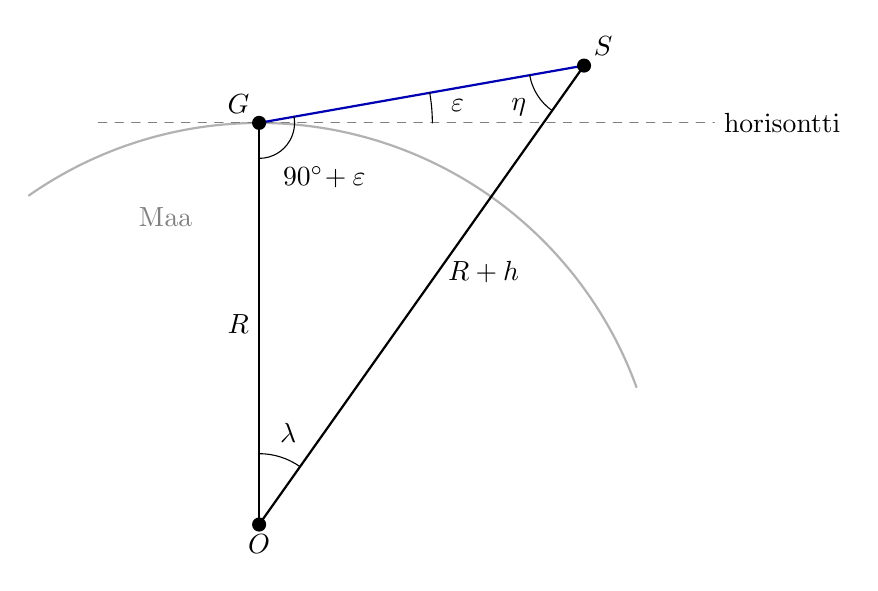
\begin{tikzpicture}[scale=1.7, line cap=round]
  % Mittakaava: R = 3, h = 1.2 (korkeus liioiteltu), epsilon = 10 deg
  % => eta = 44.7 deg, lambda = 35.3 deg; S = 4.2 (sin lambda, cos lambda)
  \coordinate (O) at (0,0);
  \coordinate (G) at (0,3);
  \coordinate (S) at (2.427,3.428);
  \coordinate (H) at (1,3);
  \draw[gray!60, thick] (125:3) arc[start angle=125, end angle=20, radius=3];
  \node[gray] at (-0.7,2.3) {Maa};
  \draw[dashed, gray] (-1.2,3) -- (3.4,3) node[right, black] {horisontti};
  \draw[thick] (O) -- (G) node[midway, left] {$R$};
  \draw[thick] (O) -- (S) node[pos=0.55, right] {$R+h$};
  \draw[thick, blue!70!black] (G) -- (S);
  \fill (O) circle (1.5pt) node[below] {$O$};
  \fill (G) circle (1.5pt) node[above left] {$G$};
  \fill (S) circle (1.5pt) node[above right] {$S$};
  \pic[draw, angle radius=0.9cm, "$\lambda$", angle eccentricity=1.35] {angle=S--O--G};
  \pic[draw, angle radius=0.7cm, "$\eta$", angle eccentricity=1.4] {angle=G--S--O};
  \pic[draw, angle radius=2.2cm, "$\varepsilon$", angle eccentricity=1.15] {angle=H--G--S};
  \pic[draw, angle radius=0.45cm, "$90^\circ\!+\varepsilon$", angle eccentricity=2.4] {angle=O--G--S};
\end{tikzpicture}
\caption{Näkyvyysgeometria. Asema $G$ näkee satelliitin $S$ elevaatiolla $\varepsilon$, kun satelliitti on keskuskulman $\lambda$ päässä asemasta. Korkeus $h$ on piirretty liioiteltuna.}
\label{fig:kolmio}
\end{figure}

\begin{enumerate}
  \item Aseman kohdalla kulma sivujen $GO$ ja $GS$ välillä on $90^\circ + \varepsilon$, koska $GO$ osoittaa suoraan alas ja $GS$ on $\varepsilon$ horisontin yläpuolella.
  \item Sinilause kolmiossa $OGS$:
  \[
  \frac{R}{\sin\eta} = \frac{R+h}{\sin(90^\circ+\varepsilon)} = \frac{R+h}{\cos\varepsilon}.
  \]
  \item Ratkaistaan nadirkulma:
  \[
  \sin\eta = \frac{R\cos\varepsilon}{R+h}.
  \]
  \item Kolmion kulmien summa on $180^\circ$:
  \[
  \lambda = 180^\circ - (90^\circ+\varepsilon) - \eta = 90^\circ - \varepsilon - \eta.
  \]
  \item Satelliitti on maskin yläpuolella, kun se on keskuskulman $\lambda$ sisällä asemasta. Pisin ylilento kulkee zeniitin kautta ja kattaa kulman $2\lambda$.
  \item Jos Maan pyörimistä ei huomioida, satelliitti kulkee kulmanopeudella $n = 2\pi/P$:
  \[
  T \approx \frac{2\lambda}{n} = \frac{2\lambda}{360^\circ}\,P.
  \]
  \item Konservatiivinen yläraja: Maa pyörii kulmanopeudella $\omega_E \approx 0,2507^\circ/\text{min}$, ja asema voi pahimmillaan liikkua samaan suuntaan kuin satelliitti. Suhteellinen kulmanopeus on silloin vähintään $n - \omega_E$:
  \[
  T_\text{max} = \frac{2\lambda}{n-\omega_E}.
  \]
\end{enumerate}

\paragraph{Numeroesimerkki: ISS} ($h \approx 425$~km apogeumissa, $\varepsilon = 10^\circ$, $R = 6378,135$~km):
\begin{align*}
\sin\eta &= \frac{6378,135\cdot\cos 10^\circ}{6802,7} = 0,9233 \quad\Rightarrow\quad \eta = 67,42^\circ,\\
\lambda &= 90^\circ - 10^\circ - 67,42^\circ = 12,58^\circ,\\
n &= 360^\circ/92,96\ \text{min} = 3,873^\circ/\text{min},\\
T &\approx \frac{2\cdot 12,58^\circ}{3,873^\circ/\text{min}} = 6,50\ \text{min},\\
T_\text{max} &= \frac{25,16^\circ}{(3,873-0,251)^\circ/\text{min}} = 6,95\ \text{min}.
\end{align*}

\paragraph{Sentinel-2B} ($h \approx 787$~km): $\lambda = 18,76^\circ$, $T \approx 10,49$~min, $T_\text{max} = 11,28$~min. Työkalun pisin laskettu Sentinel-2B-ylilento Helsingissä on 10~min 28~s, eli melkein täsmälleen pyörimättömän Maan arvio. Se on järkevää, koska polaariradalla Maan pyöriminen on lähes kohtisuorassa satelliitin liikkeeseen nähden. Testi \koodi{test\_physical\_constraints} tarkistaa, ettei mikään ylilento ylitä rajaa $T_\text{max}$.

Horisonttiin asti ($\varepsilon = 0^\circ$) ISS:n $\lambda$ on $20,4^\circ$ ja kesto noin 10,5~min. Tämä näyttää, kuinka paljon minimielevaatio lyhentää yhteysikkunaa.

Kuva~\ref{fig:taivas} näyttää yhden lähes zeniitin kautta kulkevan Sentinel-2B-ylilennon taivaskarttana.

\begin{figure}[ht]
\centering
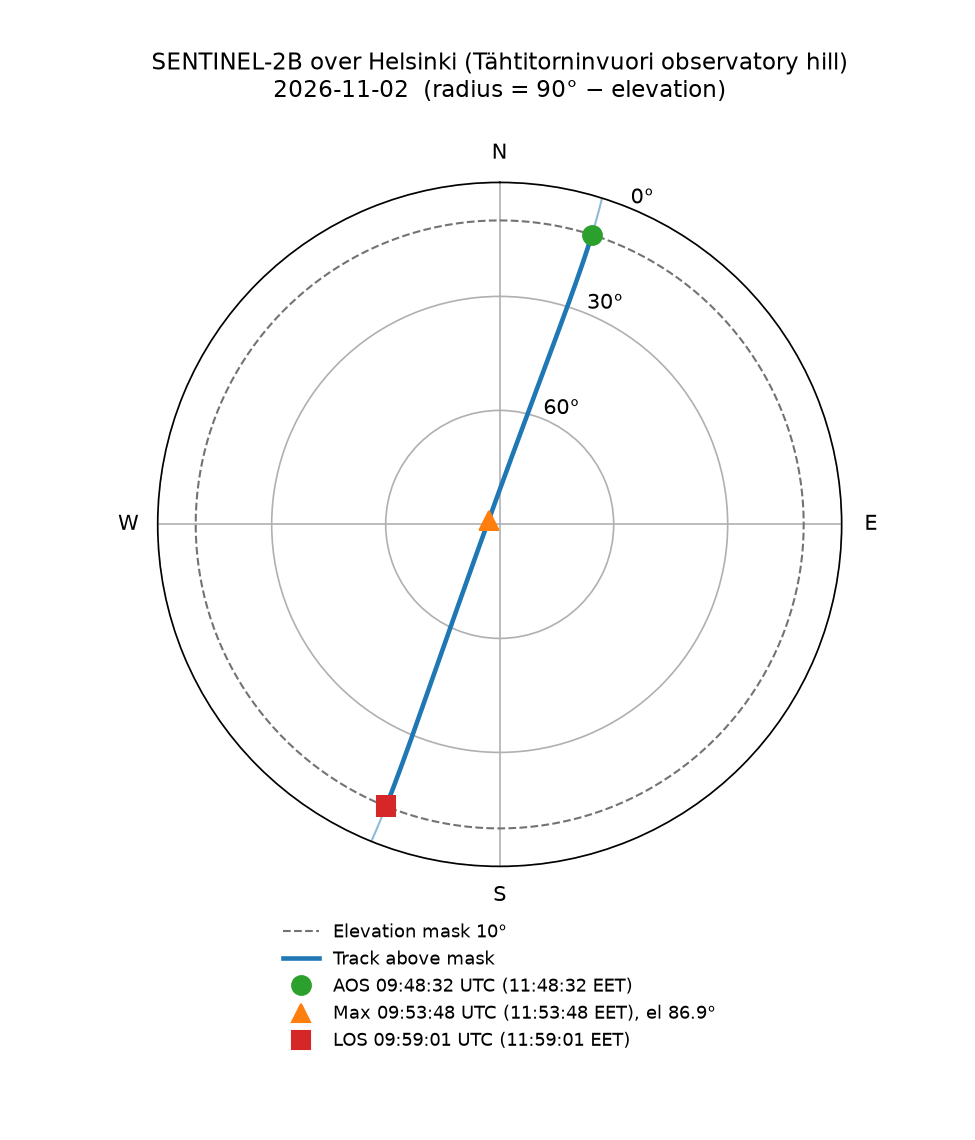
\includegraphics[width=0.62\textwidth]{images/sentinel2b_helsinki.png}
\caption{Sentinel-2B:n ylilento Helsingin yli 2.11.2026 (työkalun \koodi{--plot}-tuloste). Kulma on atsimuutti (pohjoinen ylhäällä, itä oikealla), säde on $90^\circ - E$: zeniitti on keskellä ja horisontti reunalla. Katkoviiva on 10°:n maski.}
\label{fig:taivas}
\end{figure}

\subsection{Miksi peräkkäiset ylilennot siirtyvät}

Yhden kierroksen ($\approx 93$~min ISS:llä) aikana Maa kääntyy itään
\[
\omega_E \cdot P \approx 0,2507^\circ/\text{min}\cdot 93\ \text{min} \approx 23^\circ.
\]
Seuraava maarata on siis $23^\circ$ lännempänä. Siksi ylilennot tulevat ryppäinä: muutama peräkkäinen kierros osuu asemalle (ensin idempää, sitten lännempää), ja sitten tulee monen tunnin tauko, kunnes Maa on kääntynyt niin, että rata kulkee taas lähellä.

Ryppään sisällä huippujen väli on lähellä kiertoaikaa. ISS:n kiinteällä testidatalla väli oli $1,032\,P$ ja Sentinel-2B:n $0,97$–$0,99\,P$. Testi \koodi{test\_pass\_repetition\_matches\_orbital\_period} tarkistaa, että peräkkäisillä kierroksilla $|\text{väli} - P| < T_\text{max}$.

\subsection{Miksi polaariradan satelliitti näkyy Suomesta usein}

Aurinkosynkronisen radan inklinaatio on noin $98^\circ$ (Sentinel-2B: $98,57^\circ$), eli se kulkee lähes napojen yli. Kaikki radat leikkaavat napa-alueiden läheltä, joten korkeilla leveyksillä peräkkäiset maaradat ovat lähellä toisiaan.

Sentinel-2B:n kiertoaika on 100,6~min, joten vierekkäiset maaradat ovat $\omega_E P \approx 25^\circ$ pituusastetta erillään. Päiväntasaajalla se on noin 2\,800~km, leveydellä $60^\circ$ vain noin 1\,400~km ($\cos 60^\circ = 0,5$). Näkyvyysympyrän säde on Sentinel-2B:lle 10°:n maskilla $\lambda \approx 18,8^\circ \approx 2\,100$~km. Siksi Helsingistä näkyy usea peräkkäinen kierros: kahdessa päivässä 15 ylilentoa (vertaa ISS:n 7).

ISS:n inklinaatio on $51,6^\circ$, joten sen maarata ei koskaan ulotu Helsingin leveydelle ($60,16^\circ$). Siksi ISS näkyy Helsingistä aina eteläisellä taivaalla, eikä sen elevaatio testijaksolla nouse yli $20^\circ$:n.

%----------------------------------------------------------------------
\section{Minimielevaatio (horisonttimaski)}

Yhteyttä ei yritetä aivan horisonttiin asti, koska:
\begin{itemize}
  \item \textbf{Maasto ja rakennukset} peittävät horisontin. Todellinen maski riippuu atsimuutista, ja paikalla mitattua maskia kutsutaan horisonttiprofiiliksi.
  \item \textbf{Ilmakehä}: matalalla signaali kulkee pitkän matkan ilmakehässä. Vaimennus ja tuikinta (scintillaatio) kasvavat, erityisesti korkeilla taajuuksilla (Ka-kaista, sateen vaimennus). Myös taittuminen kasvaa lähellä horisonttia \unverified[, yleistieto].
  \item \textbf{Etäisyys}: ISS:n etäisyys on zeniitissä 420~km, mutta 10°:n elevaatiolla noin 1\,500~km (Heavens-Above näyttää ISS:lle 1\,510~km). Vapaan tilan vaimennus kasvaa etäisyyden neliössä, joten $1510/420 \approx 3,6$-kertainen etäisyys tarkoittaa $20\log_{10}3,6 \approx 11$~dB heikompaa signaalia.
  \item \textbf{Antenni ja häiriöt}: maaheijastukset ja maanpinnan lämpökohina nostavat kohinalämpötilaa matalalla.
\end{itemize}
Tyypillinen arvo on 5–10° \unverified, ja tämän työkalun oletus on 10°.

%----------------------------------------------------------------------
\section{AOS, LOS, TCA ja yhteysikkuna}

\begin{itemize}
  \item \textbf{AOS} (\emph{acquisition of signal}): satelliitti nousee maskin yläpuolelle, ja yhteys voidaan aloittaa.
  \item \textbf{LOS} (\emph{loss of signal}): satelliitti laskee maskin alle, ja yhteys katkeaa.
  \item \textbf{TCA} (\emph{time of closest approach}): satelliitti on lähimpänä asemaa. Ympyräradalla tämä on käytännössä sama kuin suurimman elevaation hetki. Työkalu ilmoittaa suurimman elevaation hetken (Skyfieldin ”culminate”).
\end{itemize}

\textbf{Yhteysikkuna} AOS–LOS on maa-asematoiminnan perusyksikkö. Sen aikana:
\begin{itemize}
  \item \textbf{Ylöslinkki} (\emph{uplink}): lähetetään komennot ja aikataulutetut tehtävät, esimerkiksi ”kuvaa tämä alue”, ratamanööverin parametrit tai ohjelmistopäivitys.
  \item \textbf{Alaslinkki} (\emph{downlink}):
  \begin{itemize}
    \item telemetria (\emph{housekeeping}): lämpötilat, akkujännitteet, asento ja virheloki
    \item hyötykuorman data, esimerkiksi kuvat. Tämä on usein suurin datamäärä.
  \end{itemize}
  \item \textbf{Etäisyysmittaus} (\emph{ranging}) ja Doppler-mittaus, joita voidaan käyttää ratamääritykseen (luku~\ref{sec:od}).
\end{itemize}

Ikkunan pituus rajaa datamäärää: $10\ \text{Mbit/s} \times 8\ \text{min} \approx 4,8$~Gbit. Siksi operaatioissa suunnitellaan, mitkä ylilennot käytetään ja kenelle (projektin laajennus \koodi{passplan.schedule}, yhteysaikataulu). Käytännössä myös AOS:n ja LOS:n tarkkuudella on väliä: antennin pitää osoittaa oikeaan suuntaan ennen AOS:ia. Muutaman sekunnin virhe on yleensä harmiton, mutta minuuttien virhe hukkaa osan ikkunasta.

%----------------------------------------------------------------------
\section{Näkyykö satelliitti silmällä?}\label{sec:nakyvyys}

Ylilento on geometriaa: satelliitti on horisontin yläpuolella. Se, näkyykö satelliitti silmällä, on eri kysymys. Satelliitti ei loista itse, vaan heijastaa auringonvaloa. Se näkyy siis vain, jos kaksi ehtoa täyttyy yhtä aikaa (Skyfield-dokumentaatio: ”A satellite is generally only visible to a ground observer when there is still sunlight up at its altitude.”):
\begin{enumerate}
  \item \textbf{Satelliitti on auringonvalossa}, eikä Maan varjossa.
  \item \textbf{Havaitsijan taivas on tumma.} Työkalu vaatii, että Aurinko on yli 6° horisontin alapuolella. Raja on oma valintani (siviilihämärän loppu), ei standardi.
\end{enumerate}

Talvi-iltana Suomessa Aurinko on syvällä horisontin alla, mutta satelliitin korkeudella (400–800~km) auringonvalo ulottuu vielä pitkälle Maan yöpuolelle. Siksi illan ja aamun ylilennot ovat usein näkyviä. Keskiyön ylilennoilla satelliitti on yleensä Maan varjossa. Silloin se on taivaalla, mutta pimeänä, ja planetaario-ohjelmat merkitsevät tällaisen ylilennon esimerkiksi ”night pass -- not visible”. Nousu, huippu ja lasku ovat silti todellisia: maa-asema saisi radioyhteyden normaalisti, koska radiolinkki ei tarvitse valoa.

\paragraph{Miten varjo lasketaan.} Skyfieldin \koodi{is\_sunlit()} pitää satelliittia varjossa, jos suora satelliitista Aurinkoon osuu pallon muotoiseen Maahan (Skyfieldin lähdekoodi, versio 1.54). Koska Aurinko on hyvin kaukana, valonsäteet ovat käytännössä yhdensuuntaisia ($R_E/1\,\text{au} \approx 4\cdot10^{-5}$~rad), ja varjo on lieriö, jonka säde on Maan säde. Ehto voidaan kirjoittaa satelliitin paikkavektorilla $\mathbf r$ ja Auringon suuntaisella yksikkövektorilla $\hat s$:
\[
\text{varjossa} \iff \mathbf r\cdot\hat s < 0 \quad\text{ja}\quad |\mathbf r\times\hat s| < R_E .
\]
Ensimmäinen ehto sanoo, että satelliitti on Maan yöpuolella. Toinen sanoo, että se on lähempänä Maan ja Auringon välistä akselia kuin yhden Maan säteen päässä. Testit laskevat tämän itse ja vertaavat Skyfieldiin.

Malli on yksinkertaistus: siinä ei ole puolivarjoa eikä ilmakehää. Varjoon meno ja sieltä poistuminen voivat siksi heittää muutaman sekunnin. Silti ISS:n ylilennolla 1.11.2026 työkalun ”poistuu varjosta” -hetki oli 02:24:45 UTC, täsmälleen sama kuin Heavens-Abovella.

\paragraph{Esimerkki planetaario-ohjelman kanssa.} Cosmos 1833:n ylilennolla 31.10.2026 Sky Safari ja työkalu antoivat nousun, huipun ja laskun noin minuutin sisällä toisistaan, mutta radan muoto erosi selvästi: huippuelevaatio oli 4,5° ja 25,6°. Työkalun ratatieto oli 0,65~vrk vanha, mikä vastaa noin kilometrin virhettä eli sekunnin murto-osia. Minuutin ero tarkoittaa noin 400~km radalla, joten todennäköisin syy on, että sovelluksen ratatiedot olivat vanhoja. Tämä on käytännön esimerkki luvun~\ref{sec:tle} opetuksesta: ennuste on vain niin hyvä kuin sen ratatieto, ja vertailussa ratatiedon, paikan ja horisonttirajan pitää olla samat.

%----------------------------------------------------------------------
\section{Ratojen määritys ja ratatiedon synty: pienimmän neliösumman sovitus}\label{sec:od}

Ratojen määritys (\emph{orbit determination}, OD) tarkoittaa, että satelliitin rata estimoidaan havainnoista. Havaintoja tuottavat:
\begin{itemize}
  \item tutkat: etäisyys, suunta ja etäisyyden muutosnopeus
  \item optiset teleskoopit: suunta tähtitaustaa vasten
  \item satelliitin oma GNSS-vastaanotin
  \item maa-aseman etäisyys- ja Doppler-mittaukset
\end{itemize}

Kyse on samasta asiasta kuin data-analyysin parametrien estimoinnissa:
\begin{enumerate}
  \item \textbf{Malli}: SGP4 antaa havaittavan suureen (esim.\ suunnan tutkalta) ajan ja parametrien funktiona: $\hat y_i = f(t_i;\,\mathbf x)$, missä $\mathbf x = (n, e, i, \Omega, \omega, M, B^*)$ on ratatiedon (TLE:n tai OMM:n) sisältö.
  \item \textbf{Havainnot} $y_i$ ja niiden epävarmuudet $\sigma_i$.
  \item \textbf{Kustannusfunktio}: residuaalien painotettu neliösumma
  \[
  \chi^2(\mathbf x) = \sum_i \frac{\bigl(y_i - f(t_i;\mathbf x)\bigr)^2}{\sigma_i^2}.
  \]
  \item \textbf{Minimointi}: malli on epälineaarinen, joten se linearisoidaan alkuarvauksen ympärillä (Jacobin matriisi $H = \partial f/\partial \mathbf x$) ja parannusta haetaan iteratiivisesti (Gauss–Newton). Ratamekaniikassa tätä kutsutaan nimellä \emph{differential correction} \unverified[: termi yleisesti käytössä; Vallado 2006 mainitsee sen ohimennen].
  \item \textbf{Tulos}: parhaat parametrit sekä kovarianssimatriisi $(H^{\mathsf T} W H)^{-1}$, missä $W$ on painomatriisi ($1/\sigma_i^2$ diagonaalilla). Kovarianssi kertoo parametrien epävarmuuden.
\end{enumerate}

Ratatieto on siis SGP4-mallin parametrien sovitus tietyn aikavälin (\emph{fit span}) havaintoihin, ja epookki on sovituksen referenssihetki. Siksi sitä ei pidä käyttää muun mallin kanssa (luku~\ref{sec:tle}), ja siksi ennuste huononee nopeasti sovitusvälin ulkopuolella. Valladon mukaan sovitusvälin ulkopuolella ”the results diverge very rapidly”. Kyse on ekstrapoloinnista, ja jokainen data-analyytikko tietää, mitä se tekee sovitukselle.

Julkisia ratatietoja ei saa kovarianssin kanssa, joten niiden epävarmuutta ei tiedä suoraan. Tämä on yksi syy, miksi operaattorit tekevät omaa ratamääritystä tarkemmilla malleilla.

%----------------------------------------------------------------------
\section{Mitä tämän projektin tarkistukset osoittavat}\label{sec:tarkistukset}

Tuloksia tarkistetaan kolmella tavalla: riippumattomalla toisella toteutuksella,
fysikaalisilla rajoilla ja vertailulla kahteen muuhun ohjelmaan. Kaksi ensimmäistä ovat
automaattisia testejä (69 kpl, kansio \koodi{tests/}).

\paragraph{Testit ajetaan kiinteällä datalla.} Testit eivät hae mitään verkosta. Ne
käyttävät ratatietoja, jotka on haettu CelesTrakista kerran (31.10.\ ja 5.11.2026) ja
tallennettu kansioon \koodi{tests/data/}. Useimmat testit laskevat lisäksi kiinteälle
ikkunalle 1.11.2026 klo 00 UTC + 2~vrk. Siksi jokainen ajo antaa täsmälleen saman tuloksen
millä tahansa koneella, eikä testi riipu siitä, mitä CelesTrak juuri nyt jakaa. Testin
vertailuarvo ei koskaan tule testattavasta koodista itsestään, ja jokaisen testin kuvaus
kertoo, mistä sen vertailuarvo on peräisin.

\subsection{Riippumaton toinen toteutus}
Tiedosto \koodi{tests/reference\_geometry.py} laskee saman asian toisella tavalla.
\begin{itemize}
  \item Koordinaattimuunnokset satelliitista atsimuutiksi ja elevaatioksi (luku~\ref{sec:koord})
    on kirjoitettu itse pelkällä NumPylla, ilman Skyfieldiä: kierto TEME:stä Maahan
    kiinnitettyyn koordinaatistoon, aseman paikka WGS84-ellipsoidilla ja projektio aseman
    itä-, pohjois- ja ylös-suuntiin.
  \item Elevaatio lasketaan sekunnin välein, ja nousut ja laskut etsitään raa'asti: maskin
    ylitys interpoloidaan suoraan näytteiden välistä, ja huippu sovitetaan paraabelilla.
  \item Testit vertaavat tulosta Skyfieldin tulokseen ISS:lle ja Sentinel-2B:lle kahden
    vuorokauden ajalta. Erot ovat enintään 0,25~s nousu- ja laskuajoissa ja $0{,}002^\circ$
    elevaatiossa.
  \item Jos jommassakummassa olisi virhe, tulokset eroaisivat.
\end{itemize}
Molemmat ketjut saavat satelliitin paikan samasta SGP4:stä. SGP4:ää ei voi korvata
omalla laskulla, koska ratatieto on sovitettu juuri sille (luku~\ref{sec:tle}).
Riippumaton osa on kaikki SGP4:n jälkeen. Itse SGP4:n laskentaa projekti ei tarkista,
vaan nojaa sgp4-kirjastoon. Oma toteutus yksinkertaistaa tarkoituksella: se käyttää
Maan kiertokulmaan UTC:tä eikä UT1:tä (ero 0,09~s, luku~\ref{sec:koord}), ja siksi
aikojen toleranssi on 1~s.

\subsection{Fysikaaliset rajat}
Testit tarkistavat jokaisesta ylilennosta, että tulos on fysiikan kannalta mahdollinen:
\begin{itemize}
  \item Nousu- ja laskuhetkellä elevaatio on maskin suuruinen hakutarkkuuden rajoissa
    (elevaation muutosnopeus kertaa 0,5~s).
  \item Huippu on maskin ja $90^\circ$:n välissä.
  \item Järjestys on nousu, huippu, lasku.
  \item Ylilento ei kestä pidempään kuin geometria sallii. Enimmäiskesto $T_\text{max}$ on
    johdettu luvussa~\ref{sec:geometria}.
  \item Peräkkäiset ylilennot toistuvat kiertoajan välein.
\end{itemize}

\subsection{Vertailu muihin ohjelmiin}
Heavens-Above ja Sky Safari, neljä satelliittia ja kolme paikkaa. Menetelmä ja tulokset
ovat luvussa~\ref{sec:vertailu}. Käsin tehdyt vertailut (2.--12.11.2026) eivät kuulu
automaattisiin testeihin. Tekoälyagentin 31.10.2026 hakemista Heavens-Aboven arvoista osa
on kahdessa näkyvyystestissä vertailuarvoina.

\subsection{Yhteenveto}

\begin{center}
\small
\begin{tabularx}{\textwidth}{@{}L L L@{}}
\toprule
Tarkistus & Tulos & Mitä se osoittaa \\
\midrule
Skyfieldin elevaatio vs.\ oma NumPy-ketju (TEME $\to$ PEF $\to$ ENU), 2~vrk, 10~s välein & ero $\leq 0,0017^\circ$ (atsimuutti $\leq 0,009^\circ$) & Koordinaattimuunnokset ovat oikein (riippumattomasti toteutettu). \\
\addlinespace
Skyfieldin AOS, huippu ja LOS vs.\ raaka 1~s:n haku & AOS/LOS-ero $\leq 0,25$~s, huippu $\leq 0,11$~s, huipun elevaatio $\leq 0,002^\circ$ & Tapahtumahaku löytää kaikki ylilennot oikein ajoitettuna. \\
\addlinespace
Elevaatio AOS- ja LOS-hetkellä & = maski, enintään (elevaation muutosnopeus $\times$ 0,5~s) & Hakutoleranssi on 0,5~s, ja se näkyy oikean kokoisena. \\
\addlinespace
Kesto $\leq T_\text{max}$ (luku~\ref{sec:geometria}) & kaikki ylilennot & Kestot ovat fysikaalisesti mahdollisia. \\
\addlinespace
Huippu maskin ja $90^\circ$:n välissä, AOS $<$ huippu $<$ LOS, peräkkäiset huiput kiertoajan välein & kaikki ylilennot; väli ISS:llä $1{,}032\,P$, Sentinel-2B:llä $0{,}97$--$0{,}99\,P$ & Ylilennot ovat järkevässä järjestyksessä ja toistuvat radan tahdissa. \\
\addlinespace
Heavens-Above (ISS, Helsinki, 1.--2.11.2026; tekoälyagentin hakema) & kaikki 21 aikaa $\leq 1,1$~s, huippuelevaatiot samat asteen tarkkuudella & Ulkoinen ohjelma samalla epookilla antaa saman tuloksen. \\
\addlinespace
Käsin tehdyt vertailut 2.--12.11.2026: Heavens-Above ja Sky Safari, neljä satelliittia, kolme paikkaa (luku~\ref{sec:vertailu}) & ajat sekunnilleen tai sekunnin erolla; Sky Safarin kanssa kulmat $\leq 0{,}020^\circ$ & Kaksi muuta ohjelmaa antavat saman tuloksen eri radoilla, paikoilla ja päivinä. \\
\bottomrule
\end{tabularx}
\end{center}

Huomaa, mitä tarkistukset \textbf{eivät} osoita: ne eivät kerro, missä satelliitti oikeasti on. Kaikki vertailut käyttävät samoja ratatietoja ja samaa SGP4:ää. Todellinen virhe tulee ratatiedosta itsestään: noin kilometri epookilla, ja se kasvaa siitä. Sitä voisi mitata vain vertaamalla tarkkaan efemeridiin, esimerkiksi GPS-satelliittien tarkkoihin ratoihin (Kelso 2007 tekee näin Wikipedian mukaan).

%----------------------------------------------------------------------
\section{Kysymyksiä ja lyhyitä vastauksia}

\newcommand{\kysymys}[1]{\par\medskip\noindent\textbf{#1}\par\nopagebreak}

\kysymys{1. Mikä on TLE (tai OMM), ja miksi sitä ei voi käyttää minkä tahansa propagaattorin kanssa?}
Se on SGP4-mallin keskielementit (OMM:ssä samat luvut nimettyinä kenttinä), sovitettu havaintoihin juuri sillä mallilla. Toinen malli tulkitsee samat luvut eri tavalla. Vallado et al.\ (2006) sanoo, että jopa tilavektoriksi muuntaminen ja numeerinen integrointi on ”invalid”.

\kysymys{2. Kuinka tarkka julkinen ratatieto + SGP4 on?}
Noin kilometri epookilla, ja virhe kasvaa nopeasti, usein kilometrejä päivässä LEO:lla (arvio 1–3~km/vrk on toissijaisesta lähteestä). Tärkeintä on käyttää tuoretta ratatietoa ja tietää sen ikä. Ajoituksessa 1~km vastaa LEO:lla noin 0,13~s.

\kysymys{3. Mikä on suurin virhelähde LEO:lla?}
Ilmanvastus: ilmakehän tiheys vaihtelee Auringon aktiivisuuden mukaan, mutta SGP4:ssä on staattinen malli ja vakio $B^*$. Lisäksi ratamanööverit, joista ratatieto ei tiedä ennen kuin uusi julkaistaan.

\kysymys{4. Miten satelliitin paikasta saadaan atsimuutti ja elevaatio?}
SGP4 antaa paikan TEME-koordinaatistossa. Se kierretään Maan pyörimiskulmalla (GMST, UT1:stä) Maahan kiinnitettyyn koordinaatistoon. Näkösäde saadaan vähentämällä aseman paikka (WGS84) satelliitin paikasta, ja se projisoidaan aseman itä-, pohjois- ja ylös-vektoreille: elevaatio = arcsin(ylös-komponentti / etäisyys), atsimuutti = atan2(itä, pohjoinen).

\kysymys{5. Miksi ylilento kestää vain muutaman minuutin?}
Näkyvyysalue on pieni ja satelliitti nopea. Geometria antaa ISS:lle 10°:n maskilla keskuskulman $\lambda \approx 12,6^\circ$, ja zeniittiylilento kestää noin $2\lambda/n \approx 6,5$~min. Työkalun laskemat ISS:n ylilennot Helsingistä ovat 2–5~min.

\kysymys{6. Miksi minimielevaatio, ja mitä se maksaa?}
Maasto, ilmakehän vaimennus ja pidempi etäisyys (ISS:llä noin 11~dB huonompi linkki 10°:ssa kuin zeniitissä). Hinta on lyhyempi ikkuna: ISS:llä noin 10,5~min $\to$ 6,5~min, kun maski nousee 0°:sta 10°:een.

\kysymys{7. Miten ennusteen oikeellisuus on tarkistettu?}
Kolmella tavalla:
\begin{itemize}
  \item Riippumaton toinen menetelmä: oma koordinaattimuunnos ja raaka 1~s:n haku. Ero $< 0,3$~s.
  \item Fysikaaliset ehdot: maskin ylitys, kestoraja, kiertoaika.
  \item Ulkoiset vertailut: tekoälyagentti Heavens-Aboveen 31.10. (ero $\leq 1,1$~s) ja
    projektin tekijä käsin Heavens-Aboveen ja Sky Safariin 2.--12.11. neljällä satelliitilla kolmelta paikalta
    (ajat sekunnilleen tai sekunnin erolla). Vertailu löysi yhden virheen, joka korjattiin.
\end{itemize}
Nämä eivät todista ratatiedon omaa virhettä, eli sitä, kuinka kaukana todellinen satelliitti on ratatiedon kuvaamasta paikasta.

\kysymys{8. Mitä tapahtuu, jos ratatieto on viikon vanha?}
Paikkavirhe voi olla kymmeniä kilometrejä. Se tarkoittaa sekuntien ajoitusvirhettä (0,13~s kilometriä kohden), ja jos satelliitti on välillä tehnyt ratamanööverin, virhe voi olla paljon suurempi. Työkalu varoittaa yli 3 vuorokauden iästä. Operatiivisesti haetaan uusi ratatieto tai käytetään operaattorin omaa ratamääritystä.

\kysymys{9. Mitä tehdään, kun kahden satelliitin ylilennot menevät päällekkäin yhdellä antennilla?}
Tarvitaan aikataulu (\emph{contact scheduling}, luku~\ref{sec:aikataulu}): prioriteetit, antennin kääntymisaika ja datatarpeet. Yksinkertainen ahne sääntö toimii pienessä mittakaavassa. Oikeissa verkoissa käytetään optimointia (esim.\ kokonaislukuoptimointi), koska ahne valinta ei takaa parasta kokonaisuutta.

\kysymys{10. Mikä on ratojen määritys, ja miten se liittyy ratatietoon?}
Parametrien estimointia: radan parametreja säädetään, kunnes malli selittää havainnot (pienimmän neliösumman sovitus, iteratiivisesti linearisoiden). Ratatieto (TLE tai OMM) on tällaisen sovituksen tulos SGP4-mallilla. Siksi se on hyvä sovitusvälillä ja huononee ekstrapoloitaessa.

\end{document}
